\documentclass[
  bibliography=totoc,     % Literatur im Inhaltsverzeichnis
  captions=tableheading,  % Tabellenüberschriften
  titlepage=firstiscover, % Titelseite ist Deckblatt
]{scrartcl}

% Paket float verbessern
\usepackage{scrhack}

% Warnung, falls nochmal kompiliert werden muss
\usepackage[aux]{rerunfilecheck}

% unverzichtbare Mathe-Befehle
\usepackage{amsmath}
% viele Mathe-Symbole
\usepackage{amssymb}
% Erweiterungen für amsmath
\usepackage{mathtools}

% Fonteinstellungen
\usepackage{fontspec}
% Latin Modern Fonts werden automatisch geladen
% Alternativ:
%\setromanfont{Libertinus Serif}
%\setsansfont{Libertinus Sans}
%\setmonofont{Libertinus Mono}
\recalctypearea % Wenn man andere Schriftarten gesetzt hat,
% sollte man das Seiten-Layout neu berechnen lassen

% deutsche Spracheinstellungen
\usepackage{polyglossia}
\setmainlanguage{german}


\usepackage[
  math-style=ISO,    % ┐
  bold-style=ISO,    % │
  sans-style=italic, % │ ISO-Standard folgen
  nabla=upright,     % │
  partial=upright,   % ┘
  warnings-off={           % ┐
    mathtools-colon,       % │ unnötige Warnungen ausschalten
    mathtools-overbracket, % │
},                       % ┘
]{unicode-math}

% traditionelle Fonts für Mathematik
\setmathfont{Latin Modern Math}
% Alternativ:
%\setmathfont{Libertinus Math}

\setmathfont{XITS Math}[range={scr, bfscr}]
\setmathfont{XITS Math}[range={cal, bfcal}, StylisticSet=1]

% Zahlen und Einheiten
\usepackage[
locale=DE,                   % deutsche Einstellungen
separate-uncertainty=true,   % immer Fehler mit \pm
per-mode=symbol-or-fraction, % / in inline math, fraction in display math
]{siunitx}

% chemische Formeln
\usepackage[
version=4,
math-greek=default, % ┐ mit unicode-math zusammenarbeiten
text-greek=default, % ┘
]{mhchem}

% richtige Anführungszeichen
\usepackage[autostyle]{csquotes}

% schöne Brüche im Text
\usepackage{xfrac}

% Standardplatzierung für Floats einstellen
\usepackage{float}
\floatplacement{figure}{htbp}
\floatplacement{table}{htbp}

% Floats innerhalb einer Section halten
\usepackage[
section, % Floats innerhalb der Section halten
below,   % unterhalb der Section aber auf der selben Seite ist ok
]{placeins}

% Seite drehen für breite Tabellen: landscape Umgebung
\usepackage{pdflscape}

% Captions schöner machen.
\usepackage[
  labelfont=bf,        % Tabelle x: Abbildung y: ist jetzt fett
  font=small,          % Schrift etwas kleiner als Dokument
  width=0.9\textwidth, % maximale Breite einer Caption schmaler
]{caption}
% subfigure, subtable, subref
\usepackage{subcaption}

% Grafiken können eingebunden werden
\usepackage{graphicx}
% größere Variation von Dateinamen möglich
\usepackage{grffile}

% schöne Tabellen
\usepackage{booktabs}

% Verbesserungen am Schriftbild
\usepackage{microtype}

% Literaturverzeichnis
\usepackage[style=alphabetic,]{biblatex}
% Quellendatenbank
\addbibresource{lit.bib}

% Hyperlinks im Dokument
\usepackage[
  unicode,        % Unicode in PDF-Attributen erlauben
  pdfusetitle,    % Titel, Autoren und Datum als PDF-Attribute
  pdfcreator={},  % ┐ PDF-Attribute säubern
  pdfproducer={}, % ┘
]{hyperref}
% erweiterte Bookmarks im PDF
\usepackage{bookmark}

% Trennung von Wörtern mit Strichen
\usepackage[shortcuts]{extdash}

\title{V351: Fourier-Analyse und Synthese}
\author{
  Simon Schulte
  \texorpdfstring{
    \\
    \href{mailto:simon.schulte@udo.edu}{simon.schulte@udo.edu}
  }{}
  \texorpdfstring{\and}{, }
  Tim Sedlaczek
  \texorpdfstring{
    \\
    \href{mailto:tim.sedlaczek@udo.edu}{tim.sedlaczek@udo.edu}
  }{}
}
\publishers{TU Dortmund – Fakultät Physik}

\date{Durchführung: 17.1.2017\\
      Abgabe: 24.01.2016}


\begin{document}

\maketitle
\thispagestyle{empty}
\tableofcontents
\newpage
\section{Zielsetzung}
\label{zielsetzung}
Ziel des Versuchs ist es, mit Hilfe der Fourier-Analyse eine zeitlich periodische
Spannungsschwingung in ihre einzelnen Fourier-Komponenten zu zerlegen, sowie
eine solche Schwingung aus ihren Komponenten zu synthetisieren.
\section{Theorie}
\label{theorie}
Schwingungen sind räumlich oder zeitlich wiederkehrende periodische Veränderungen.
Sie treten also entweder nach einer bestimmten Periodendauer oder einer
bestimmten Entfernung wieder auf. Schwingungen lassen sich theoretisch immer
als sinus- oder cosinusfunktion beschreiben. \\
\\
Das Fouriersche Theorem versucht jede Schwingung aus einer Kombination von
sinus- und cosinusfunktionen zu charakterisieren. So lässt sich eine periodische
Funktion $f(t)$ mit der Periodendauer $T$ darstellen als:
\begin{equation}
	\frac{1}{2}a_0+\sum_{n=1}^{\infty}\left(a_n\cos\left(n\frac{2\pi}{T}t\right)+b_n\sin\left(n\frac{2\pi}{T}t\right)\right),\:\:\:n\in\mathbb{N}
	\label{fourier_theorem}
\end{equation}
$a_n$ und $b_n$ sind die Fourier-Koeffizienten. Diese lassen sich mit diesen
Gleichungen bestimmen:
\begin{align}
	a_n=&\frac{2}{T}\int_0^T f(t)\cos\left(n\frac{2\pi}{T}t\right)\mathup{d}t&\\
	b_n=&\frac{2}{T}\int_0^T f(t)\sin\left(n\frac{2\pi}{T}t\right)\mathup{d}t&n=1,2,\ldots
	\label{fourier_koeffizienten}
\end{align}
Gleichung \ref{fourier_theorem} gilt nur, falls $f(t)$ stetig ist und die
unendliche Potenzreihe gleichmäßig konvergiert. Wenn $f$ an einer Stelle nicht
stetig ist, treten Abweichungen in der Approximation durch die Fourier-Reihe
auf. Bei einer Betrachtung in einem endlichen Zeitintervall, also wenn die Reihe
nicht bis unendlich geht, ist dies für die Ränder gegeben. Deswegen treten im
Experiment Abweichungen in der Approximation auf. Dieser Effekt wird Gibbssches
Phänomen genannt.
\subsection{Fourier-Transformation}
Neben der Darstellung als Fourier-Reihe und einer Zerlegung in $n$ Schwingungen,
ist es auch möglich aus einer Funktion $f(t)$ das Frequenzspektrum zu bestimmen.
Dies wird dann als Fourier-Transformation bezeichnet. Es ist bei der Fourier-Transformation
nicht von Bedeutung, ob $f(t)$ eine periodische Funktion ist. Außerdem ist die
Fourier-Transformation umkehrbar. Es gilt:
\begin{equation}
	g(\nu)=\int_{-\infty}^{\infty}f(t)\mathup{e}^{\mathup{i}\nu t}\mathup{d}t.
	\label{fourier_trafo}
\end{equation}
Dabei ist $g(\nu)$ das Frequenzspektrum der Funktion $f(t)$. Sollte es sich bei
$f(t)$ um eine periodische Funktion handeln, besteht das Frequenzspektrum aus
Delta-Funktionen. Damit ist es dann ein diskretes Spektrum. Wenn $f(t)$ nicht
periodisch ist handelt es sich um ein kontinuierliches Spektrum. Das im Versuch
verwendete Oszilloskop ist in der Lage eine Fouriertransformation mit diskreten
Daten automatisch durchzuführen. Dabei muss das Abtasttheorem beachtet werden,
welches besagt, dass die Abtastfrequenz eines Messgerätes mindestens zweimal so
groß, wie die größte zu untersuchende Frequenz einer Oberwelle sein sollte. Wird
also bis zur $n$-ten Oberwelle untersucht, so gilt

\begin{equation}
	\nu_{\mathup{A}}>2n\nu_1,
	\label{abtasttheorem}
\end{equation}

wobei $\nu_{\mathup{A}}$ die Abtastfrequenz und $\nu_1$ die Frequenz der
Grundschwingung ist.
\subsection{Die Rechteck-, Dreieck- und Sägezahnspannung}
\label{formeln}
Es werden in dem Versuch drei verschiedene Spannungsverläufe untersucht.
Die erste untersuchte Spannung, die Rechteckspannung, wird zur Vereinfachung
als ungerade Funktion definiert. Daher gilt:

\begin{equation}
	a_n=0
\end{equation}

Es ergibt sich desweiteren:

\begin{equation}
	b_n=
	\begin{cases}
		0,  & n \:\:\mathup{gerade}\\
		\frac{4}{n\pi}, &n \:\:\mathup{ungerade}
	\end{cases}
\label{rechteck}
\end{equation}

Auch die zweite untersuchte Spannung, die Sägezahnspannung, wird als ungerade
Funktion definiert. Folglich gilt auch hier:

\begin{equation}
	a_n=0
\end{equation}

Desweiteren ergibt die Rechnung für den Koeffizienten der zweiten Summe:

\begin{equation}
	b_n=(-1)^{n+1}\frac{2}{n}
  \label{sägezahn}
\end{equation}

Die dritte untersuchte Spannung, die Dreieckspannung, wird zur Vereinfachung
als gerade Funktion definiert. Es folgt:

\begin{equation}
	b_n=0
\end{equation}

Für $a_n$ gilt:

\begin{equation}
	a_n=
	\begin{cases}
		0,  & n \:\:\mathup{gerade}\\
		-\frac{4}{n^2\pi}, &n \:\:\mathup{ungerade}
	\end{cases}
\label{dreieck}
\end{equation}
\section{Durchführung}
\subsection{Die Fourier-Analyse}
\begin{figure}[htb]
  \centering
  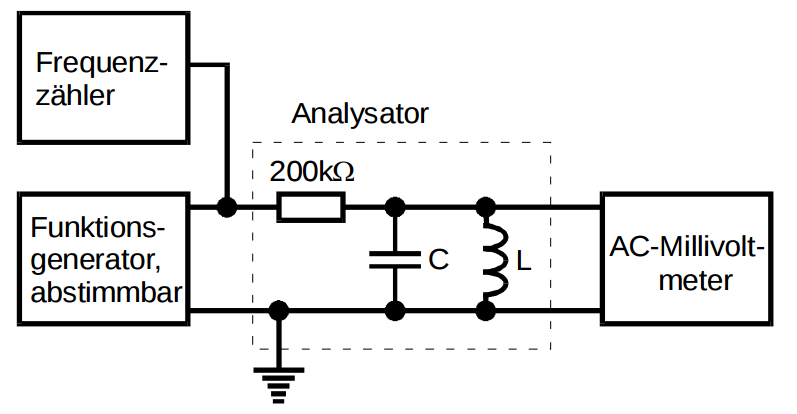
\includegraphics[width=0.75\textwidth]{V3511.png}
  \caption{Schematische Darstellung der Fourier-Analyse mit einem Speicheroszilloskop}
\end{figure}
\label{V3511}
In Abbildung \ref{V3511} ist ein regelbarer Funktionsgenerator, der mit einem
digitalen Speicheroszilloskop verbunden ist, zu sehen. Es werden zunächst drei
verschiedene periodische Spannungsverläufe in ihre Fourier-Konstanten zerlegt.
Durch das Einstellen des Math-Modus im Oszilloskop werden die Spannungsverläufe
in ihre einzelnen Frequenzen zerlegt. Dadurch können die Amplituden der
einzelnen Bestandteile abgelesen werden. Es wird am Frequenzgenerator eine
Rechteck-, eine Dreieck- und eine Sägezahnspannung erzeugt. Das Frequenzspektrum
der jeweiligen Spannung wird mit Hilfe des Oszillographen gebildet. Am
Oszilloskop können dann die einzelnen Peaks abgelesen werden und so für die
verschiedenen $n$-ten Oberwellen die Amplituden aufgenommen werden. Diese Werte
sollten dann, abhängig von der Höhe der Grundschwingung, mit den berechneten
Werten übereinstimmen.
\subsection{Die Fourier-Synthese}
Zur Synthese einer zeitlich periodischen Stromschwingung werden zu den
Frequenzen der Oberwellen jeweils die einzelnen Amplituden benötigt. Dafür kann
man die Formeln aus \ref{formeln} nutzen. Sind Frequenz und Amplitude der
benötigten Oberwelle bekannt, lässt sich die Schwingung mit Hilfe eines
Oberwellengenerators synthetisieren. Dabei werden die ersten 9 Oberwellen am
Generator eingestellt und so in Phase gebracht, dass das Ergebnis der zu
erzeugenden Spannung möglichst nahe kommt.
\end{document}
